% RNA base ==> scartato poichè c'è solo una classe
\section{Analisi dei dati}\label{sec:analisi_dati}\cite{LEZIONI}

In questa sezione avviene l'esplorazione del dataset completo, considerando diverse caratteristiche tra le quali:
\begin{itemize}
\item Ricerca di eventuali valori nulli
\item Ricerca di eventuali valori mancanti
\item valori discreti o continui
\item Tipo di dati
\item Range delle features
\item collinearità, multicollinearità dei dati
\item matrice di correlazione





\end{itemize}
\subsection{EDA: Exploratory Data Analysis}\label{ssec:EDA}

Il dataset è composto da 28 features metre, come mezionato precedentemente, la target label è stata classificata in 4 classi da un team di medici egiziani. Sono stati campionati in tutto 1385 samples, ogni sample contiene i dati del paziente.
Per avere un'informazione dettagliata e precisa dei dati sono state impigate le funzioni di pandas tra le quali: pandas.describe() e pandas.info(). Tutte e due le funzioni prendono in input il dataset completo e mentre la prima descrive la tipologia dei dati e il conteggio di essi, la seconda dà inforazioni riguardanti diversi ulteriori parametri come la media per ogni features, il minimo, il massimo valore e i percentili.  
Analizzando il dataset attraverso questi metodi, non ci sono valori nulli/mancanti nè feature duplicate e i tipi di dati sono int e float. 


\begin{table}[ht]
\centering
\begin{tabular}{|l|l|l|l|l|} 
\hline
\rowcolor{black}                                            & \textcolor{white}{\textbf{\textit{RNA EOT}}} & \textcolor{white}{\textbf{\textit{RNA 12}}} & \begin{tabular}[c]{@{}>{\cellcolor{black}}l@{}}\textcolor{white}{\textbf{Baseline histological }}\\\textcolor{white}{\textbf{Grading}}\end{tabular} & \begin{tabular}[c]{@{}>{\cellcolor{black}}l@{}}\textcolor{white}{\textbf{\textit{Baseline histological }}}\\\textcolor{white}{\textbf{\textit{Grading}}}\end{tabular}  \\ 
\hline
\rowcolor{black} \textcolor{white}{\textbf{\textit{count}}} & \textcolor{white}{\textbf{1385}}             & \textcolor{white}{\textbf{1385}}            & \textcolor{white}{\textbf{1385}}                                                                                                                    & \textcolor{white}{\textbf{1385}}                                                                                                                                       \\ 
\hline
\rowcolor{black} \textcolor{white}{\textbf{\textit{mean}}}  & \textcolor{white}{\textbf{287660.336462}}    & \textcolor{white}{\textbf{2.887536e+05}}    & \textcolor{white}{\textbf{~9.761733~}}                                                                                                              & \textcolor{white}{\textbf{2.536462}}                                                                                                                                   \\ 
\hline
\rowcolor{black} \textcolor{white}{\textbf{\textit{std}}}   & \textcolor{white}{\textbf{264559.525070}}    & \textcolor{white}{\textbf{2.853507e+05}}    & \textcolor{white}{\textbf{4.023896}}                                                                                                                & \textcolor{white}{\textbf{1.121392}}                                                                                                                                   \\ 
\hline
\rowcolor{black} \textcolor{white}{\textbf{\textit{min}}}   & \textcolor{white}{\textbf{5}}                & \textcolor{white}{\textbf{5}}               & \textcolor{white}{\textbf{3}}                                                                                                                       & \textcolor{white}{\textbf{1}}                                                                                                                                          \\ 
\hline
\rowcolor{black} \textcolor{white}{\textbf{\textit{25\%}}}  & \textcolor{white}{\textbf{5}}                & \textcolor{white}{\textbf{5}}               & \textcolor{white}{\textbf{6}}                                                                                                                       & \textcolor{white}{\textbf{2}}                                                                                                                                          \\ 
\hline
\rowcolor{black} \textcolor{white}{\textbf{\textit{50\%}}}  & \textcolor{white}{\textbf{251376}}           & \textcolor{white}{\textbf{2.343590e+05}}    & \textcolor{white}{\textbf{10}}                                                                                                                      & \textcolor{white}{\textbf{3}}                                                                                                                                          \\ 
\hline
\rowcolor{black} \textcolor{white}{\textbf{\textit{75\%}}}  & \textcolor{white}{\textbf{517806}}           & \textcolor{white}{\textbf{5.248190e+05}}    & \textcolor{white}{\textbf{13}}                                                                                                                      & \textcolor{white}{\textbf{4}}                                                                                                                                          \\ 
\hline
\rowcolor{black} \textcolor{white}{\textbf{\textit{max}}}   & \textcolor{white}{\textbf{808450}}           & \textcolor{white}{\textbf{3.731527e+06}}    & \textcolor{white}{\textbf{16}}                                                                                                                      & \textcolor{white}{\textbf{4}}                                                                                                                                          \\
\hline
\end{tabular}
\caption{Alcuni valori estratti da pandas.describe()}
\end{table}

I valori delle features nel caso di RBC, AST, ALT, RNA sono valori continui, mentre alcuni valori come Nausea, Diarrea, Età sono valori discreti. In accordo con le \textbf{raccomandazioni dei medici} mostrate nel dataset description, sono stati \textbf{discretizzati} in dei range ad hoc tutti i valori presenti di ogni feature nel dataset. Questo tipo di operazione, la discretizzazione, è stata effettuta nella fase di EDA e non di preproccessing come normalmente avverrebbe, poichè nella descrizione del dataset si suppone fin dall'inizio di avere il datast già discretizzato. Inoltre, discretizzando i dati, si possono avere dei grafici molto più indicativi dal punto di vista medico dei valori stessi delle features. Sono stati riportati i range delle features per la discretizazione.



\begin{table}[ht]\label{tab:discretization criteria}
\centering
\resizebox{0.7\textwidth}{!}{\begin{minipage}{\textwidth}
\begin{tabular}{lll}
Feature Names                 & Feature Values  & Discretization (Items)                                                                                                                                 \\
Age                           & 32:61           & {[}0; 32], ]32; 37], ]37; 42],]42; 47], ]47; 52], ]52; 57],]57; 62]                                                                                    \\
Gender                        & Male,Female     & {[}Male], [Female]                                                                                                                                     \\
BMI(Body Mass Index)          & 22:35           & {[}0; 18:5[ [18:5; 25[, [25; 30[, [30; 35[, [35; 40[                                                                                                   \\
Fever                         & Absent, Present & {[}Absent], [Present] -                                                                                                                                \\
Nausea/Vomiting               & Absent, Present & {[}Absent], [Present] -                                                                                                                                \\
Headache                      & Absent, Present & {[}Absent], [Present] -                                                                                                                                \\
Diarrhea                      & Absent, Present & {[}Absent], [Present] -                                                                                                                                \\
Fatigue                       & Absent, Present & {[}Absent], [Present] -                                                                                                                                \\
Bone ache                     & Absent, Present & {[}Absent], [Present] -                                                                                                                                \\
Jaundice                      & Absent, Present & {[}Absent], [Present] -                                                                                                                                \\
Epigastria pain               & Absent, Present & {[}Absent], [Present] -                                                                                                                                \\
WBC(White Blood Cells)        & 2991:12101      & {[}0; 4000[, [4000; 11000[, [11000; 12101]                                                                                                             \\
RBC(Red Blood Cells)          & 3816422:5018451 & {[}0; 3000000[, [3000000; 5000000[,[5000000; 5018451]                                                                                                  \\
HGB(Hemoglobin)               & 2:20            & \begin{tabular}[c]{@{}l@{}}If (Gender==[Male]):[2; 14[, [14; 17:5], ]17:5; 20]\\If(Gender==[Female]):[2; 12:3[, [12:3; 15:3], ]15:3; 20]\end{tabular}  \\
Plat(Platelet)                & 93013:226464    & {[}93013; 100000[, [100000; 255000[,[255000; 226465[                                                                                                   \\
AST1(1 week)                  & 0:128     & {[}0; 20[, [20; 40], ]40; 128]                                                                                                                         \\
ALT1(1 week)                  & 0:128      & {[}0; 20[, [20; 40], ]40; 128]                                                                                                                         \\
ALT4(4 weeks)                 & 0:128      & {[}0; 20[, [20; 40], ]40; 128]                                                                                                                         \\
ALT12(12 weeks)               & 0:128      & {[}0; 20[, [20; 40], ]40; 128]                                                                                                                         \\
ALT24(24 weeks)               & 0:128      & {[}0; 20[, [20; 40], ]40; 128]                                                                                                                         \\
ALT36(36 weeks)               & 0:128      & {[}0; 20[, [20; 40], ]40; 128]                                                                                                                         \\
ALT48(48 weeks)               & 0:128      & {[}0; 20[, [20; 40], ]40; 128]                                                                                                                         \\
RNA Base                      & 0:1201086       & {[}0; 5], ]5; 1201086]                                                                                                                                 \\
RNA 4                         & 0:1201715       & {[}0; 5], ]5; 1201715]                                                                                                                                 \\
RNA 12                        & 0:3731527       & {[}0; 5], ]5; 3731527]                                                                                                                                 \\
RNA EOT                       & 0:808450        & {[}0; 5], ]5; 808450]                                                                                                                                  \\
RNA EF(Elongation Factor)     & 0:808450        & {[}0; 5], ]5; 808450]                                                                                                                                  \\
Baseline Histological Grading & 1:16            & {[}1]; [2]; [3]; :::[16]                                                                                                                               \\
                                                     
\end{tabular}\label{tab:tab1}
\end{minipage}}
\caption{\textbf{Criteri di discretizzazione}}
\end{table}

Il dataset risulta essere bilanciato, ovvero ogni classe di fibrosi è presente in modo equamente distribuito. Questa osservazione ci fa precludere un metodo di preprocessing per ribilanciare la fase di addestramento dei modelli. Infatti avere delle classi bilanciate nel dataset farà in modo che il modello impari a distiguere le classi in modo equo, senza dare più importanza ad un tipo di fibrosi rispetto ad un altra.
\begin{figure}[H]
    \centering
    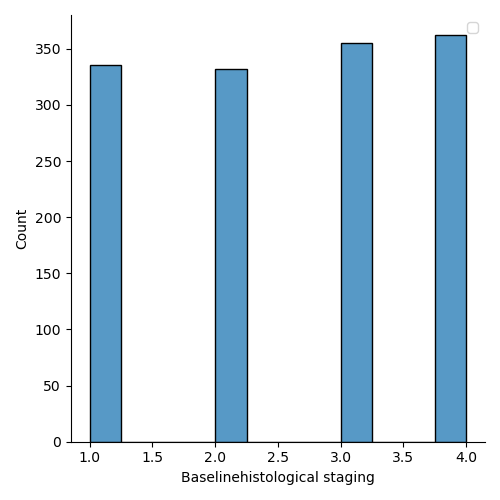
\includegraphics[width=0.5\columnwidth]{figures/target_label.png}
    \caption{Dataset bilanciato}
    \label{fig:target}
\end{figure}



E' stato affrontata l'analisi delle features, dopo la discretizzazione, ed è emerso che alcune feature assumono un solo valore del range stabilito (fig. \ref{fig:distr_features_1}) oppure la maggior parte dei sample ha lo stesso valore, fig. \ref{fig:distr_features_2}. Questo indica che sull'uscita non hanno alcun effetto poichè quello stesso valore compare sempre, indipendentemente dalla classe di output.

\begin{figure}[H]
    \centering
    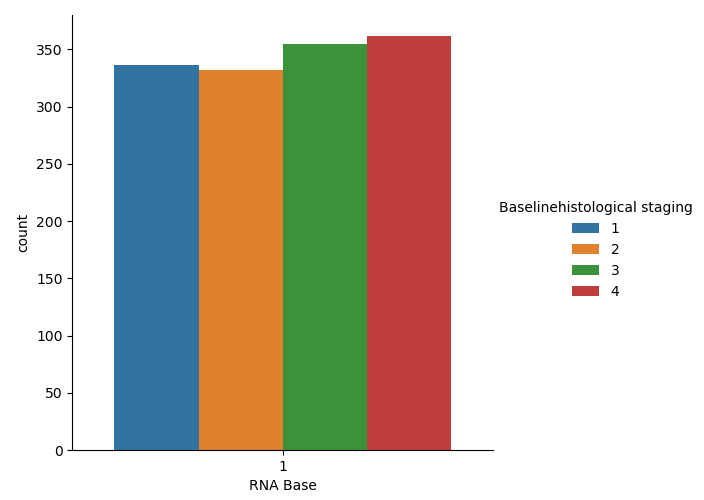
\includegraphics[width=0.4\columnwidth]{figures/RNA base.png}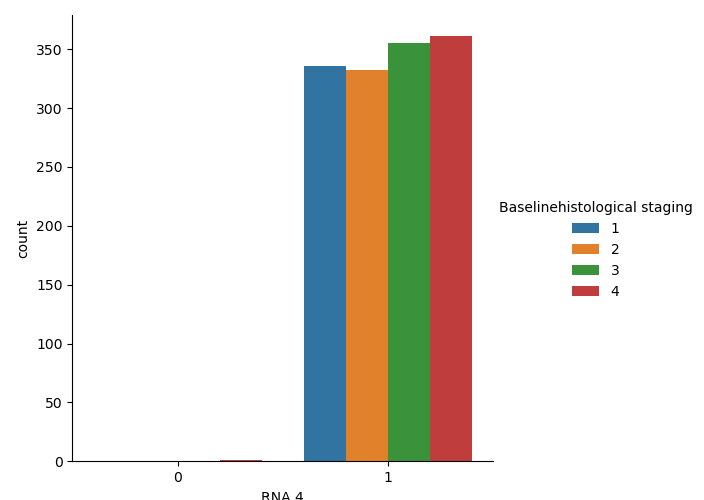
\includegraphics[width=0.4\columnwidth]{figures/RNA 4.png}
    
    \caption{Distribuzione features, un solo valore}
    \label{fig:distr_features_1}
\end{figure}

\begin{figure}[H]
    \centering
    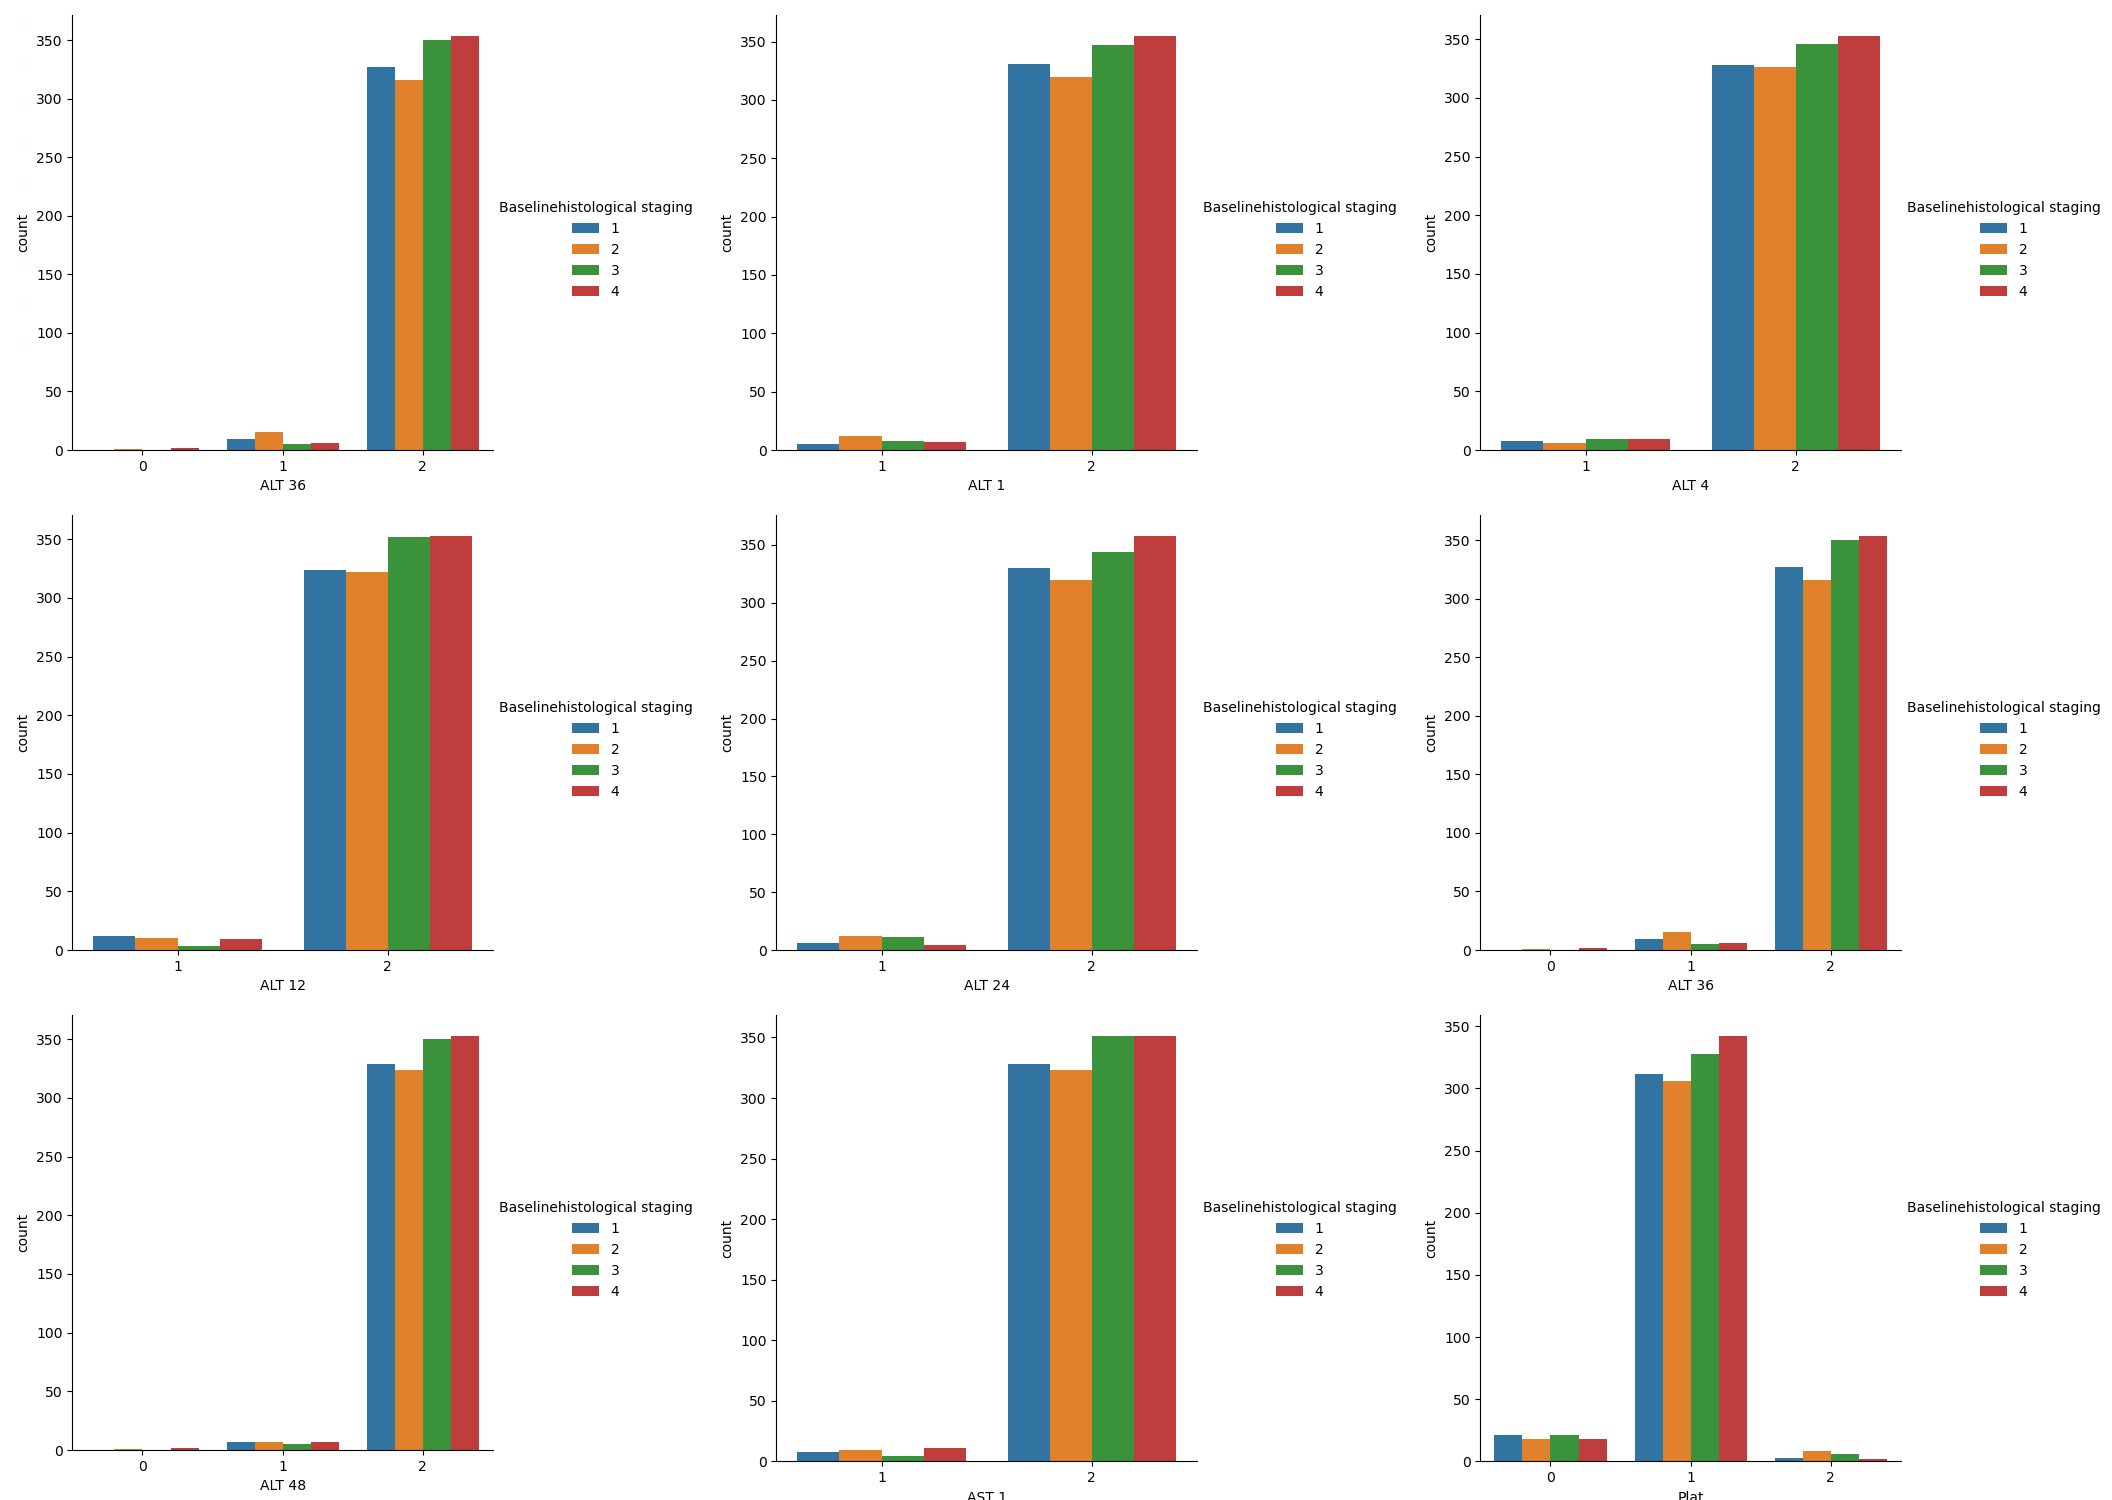
\includegraphics[width=1\columnwidth]{figures/plots_features.png}
    \caption{Distribuzione features, maggior parte dei valori in solo range}
    \label{fig:distr_features_2}
\end{figure}

\subsection{Correlazione tra le features}

Inoltre, il dataset è stato impiegato per valutare la correlazione tra ogni coppia di feature e tra le varie features e l'output target, così da evidenziare eventuali multicollinearità presenti. E' stata usata per questo scopo la matrice di correlazione. Si nota che c'è una discreta correlazione tra le features RNA 12 e RNA EOT. Ciò potrebbe far intuire che i pazienti che hanno l'RNA del virus dopo 12 settimane, probabilmente avranno un indice alto di RNA HCV anche alla fine del trattamento e che quindi sono i più predisposti alla cirrosi cronica. Questa osservazione è in linea con quanto detto precedentemente, ovvero che una volta contratto il virus sarà difficile guarire definitivamente.
Si può notare chiaramente che nessuna delle features è fortemente correlata alla classe target, per cui non c'è collinearità tra l'uscita e le features e, dunque, i metodi migliori per determinare l'output sono quelli di classificazione e non di regressione lineare.

\begin{figure}[H]
    \centering
    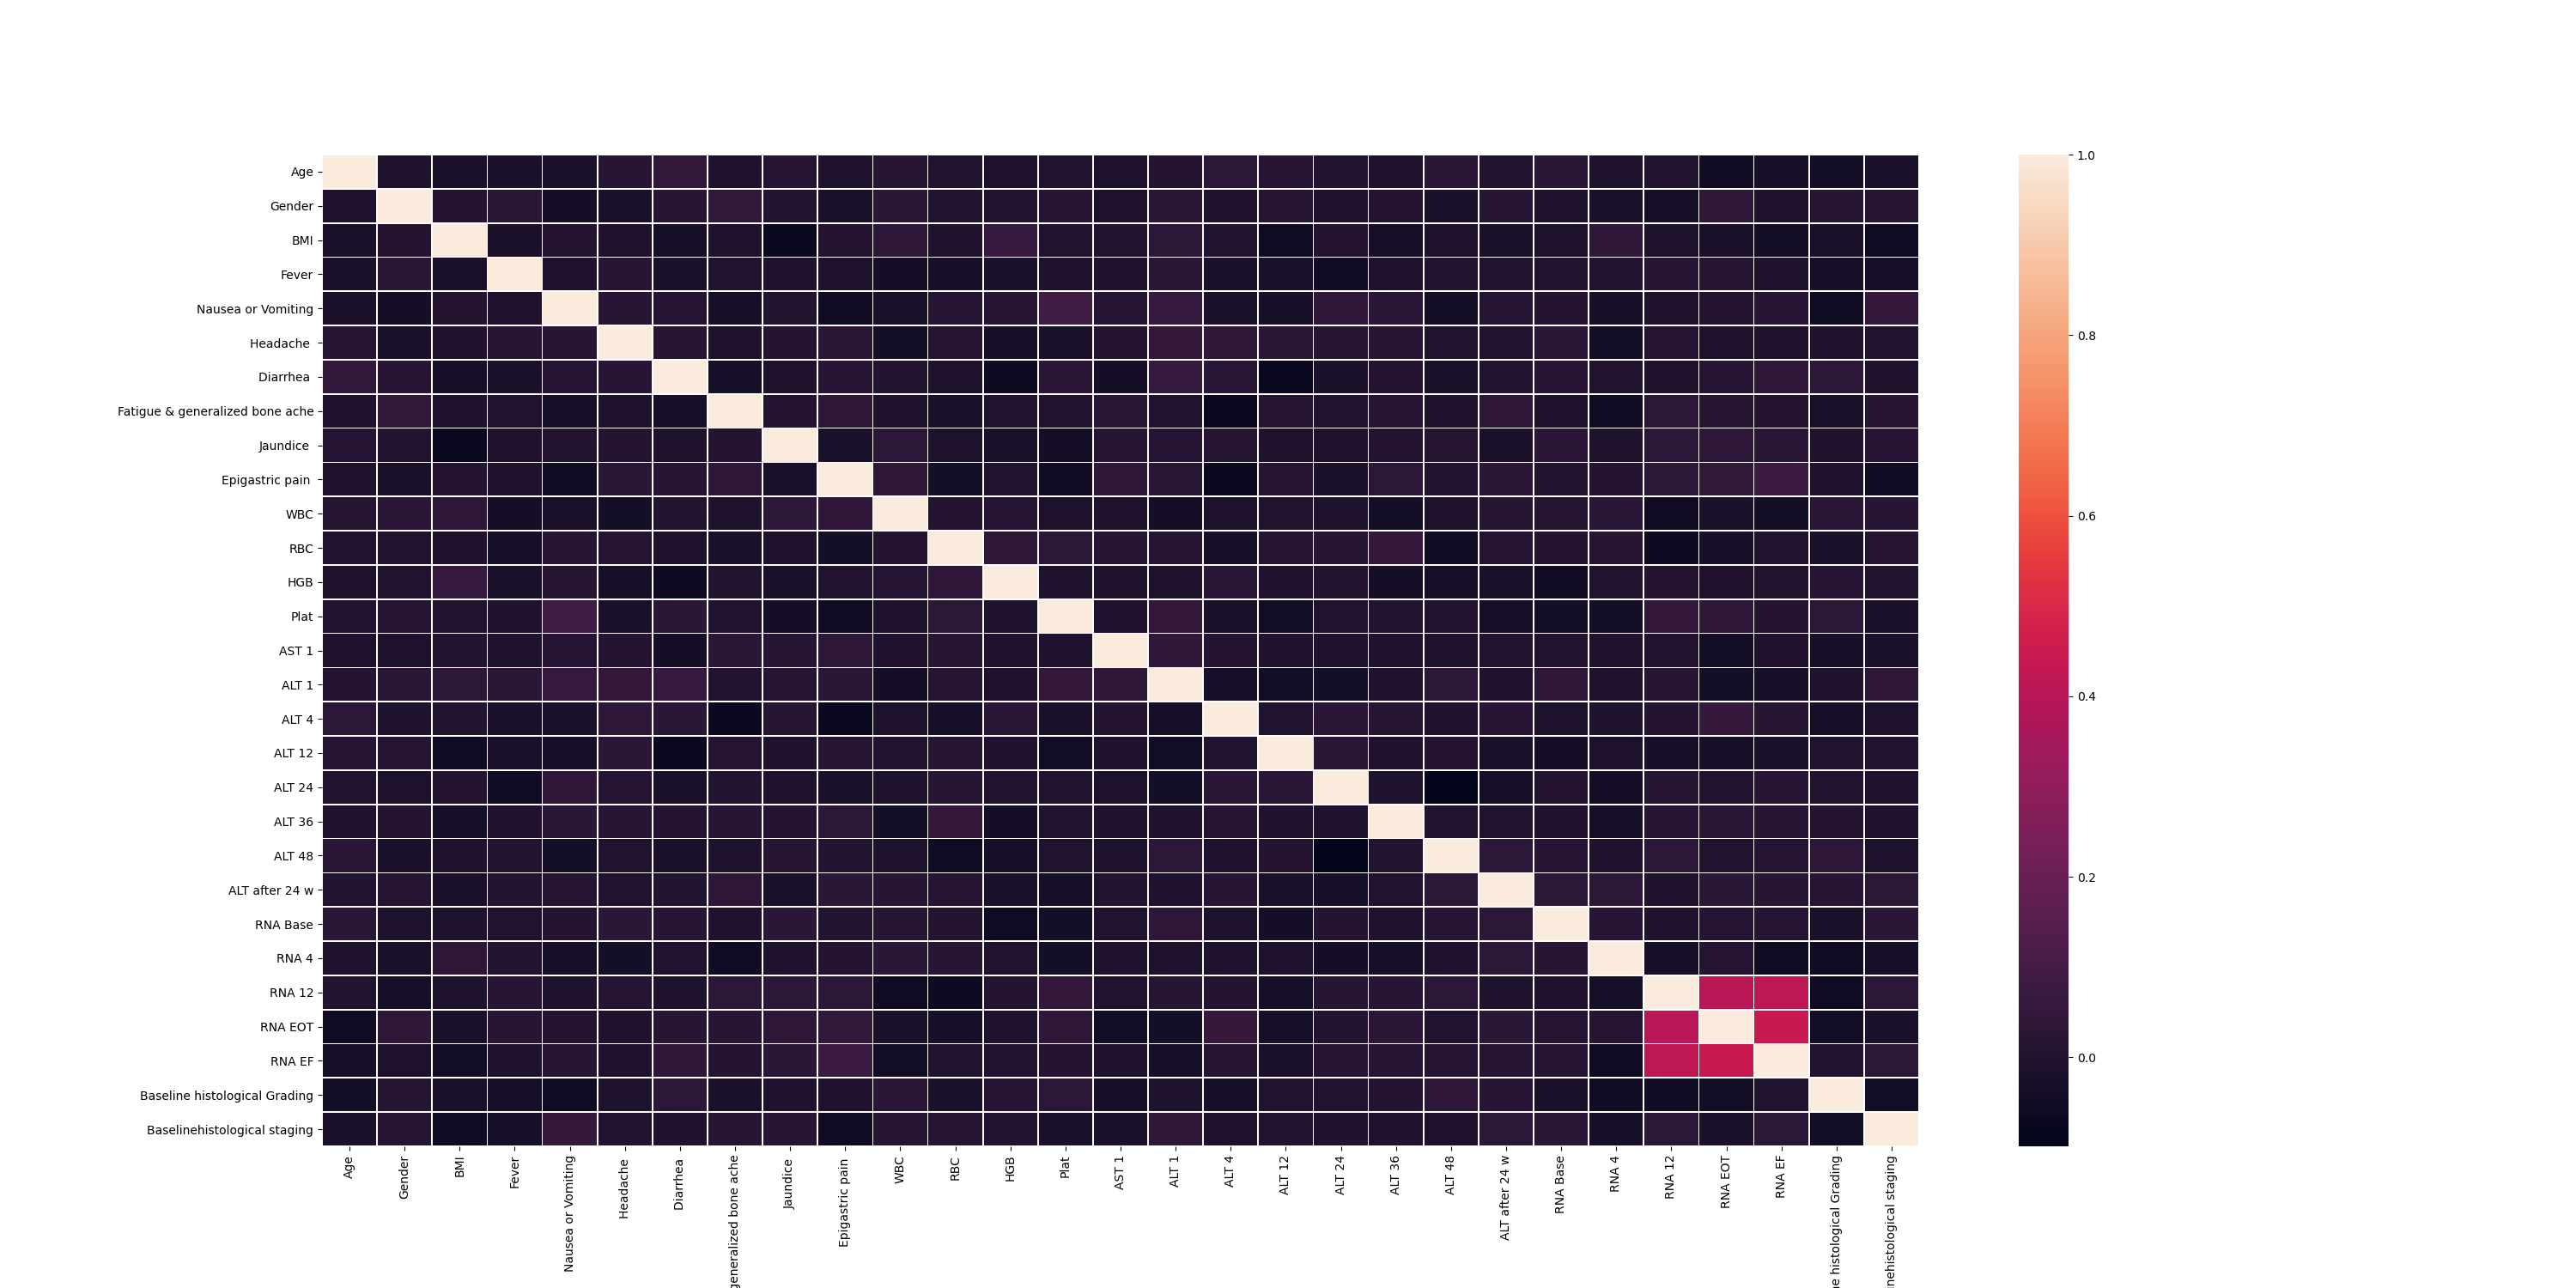
\includegraphics[width=1\columnwidth]{figures/matrx_corr.png}
    \caption{Matrice di Correlazione}
    \label{fig:matr_corr}
\end{figure}

\subsection{Clustering per valutazione della complessità del problema}

Ho voluto trattare inizialmente i dati, anche quelli non discretizzati, per avere un'idea della difficoltà di classificazione del dataset. Per questa ragione è stato usato un algoritmo di clustering su 3 features, sia discretizzate che non, (Baseline histological Grading, RNA EOT, RNA EF), che, in accordo con i medici, potrebbero ben "classificare" le 4 famiglie di fibrosi. La scelta di un numero così basso di features (3 su 28) è stato effettuato per rappresentare graficamente i dati con un numero notevolmente inferiore di features. 

Prima di tutto però, partiamo col definire cos'è il clustering. Il clustering appartiene alla famiglia degli algoritmi non supervisionati e consiste nell'etichettare una mole di dati senza conoscere l'etichette, scoprendo raggruppamenti tra dati simili tra loro. Questa tipologia di algoritmi è utilizzata sopratutto quando, come in molti dei casi reali, non si possiedono etichette e non si ha la potenza computazionale e/o il tempo per etichettare tutti i dati. Infatti i punti "simili" tra loro finiscono nello stesso gruppo, mentre quelli diversi finiscono in gruppi diversi. Per raggruppare i punti si devono considerare principalmente 2 aspetti:
\begin{itemize}
    \item Il primo è quello di misurare la distanza tra questi punti, che può essere euclidea, di Manhattan, di Mahalanobis. Ogni definizione diversa di distanza può creare cluster di diversa forma.
    \item Il secondo è quello di valutare la qualità di un clustering attraverso, per esempio, la distanza tra i baricentri di ogni cluster
\end{itemize}
I dati in questione da me utilizzati per il clustering non sono stati normalizzati o standardizzati poichè questo potrebbe influire negativamente sulla bontà del clustering e ho voluto appositamente utilizzare i dati "crudi" del dataset per evidenziare eventuali pattern nascosti. 
L'algoritmo da me utilizzato è il K-Means che cerca di minimizzare una certa funzione obbiettivo.
Prima di tutto però bisogna rappresentare un insieme di N punti attraverso un solo punto x*. Per farlo si può utilizzare il criterio della minima distanza euclidea:

\begin{equation}
    J(\mathbf{x*})=\sum_{N}^{n=1}\left \| \mathbf{x_{n}-x*}  \right \|^{2}
\end{equation}

Il minimo di questa funzione è il punto medio dei dati, ovvero il baricentro. Ecco quindi che si possono raggruppare N punti in k cluster considerando come funzione l'errore quadratico totale considerando i cluster come gli insiemi C1, C2,...,Ck e come centri i rispettivi baricentri. 
L'algoritmo in esame è il K-Means che approssima il minimo di \begin{math}J_e\end{math} definita come:

\begin{equation}
    J_{e}=\sum_{k}^{q=1}\sum_{x\epsilon C_{q}}^{}\left \| x-c_{q} \right \|^{2}
\end{equation}

Il numero di cluster scelto, k, è un iperparametro e questo sta a significare che dobbiamo sceglierlo con un buon criterio. Il metodo per trovarlo in modo oppurtuno è rappresentare il rapporto di \begin{math}J_k/J_1\end{math}, chiamata inertia, in funzione di k. Quello che è stato fatto è riportare graficamente questa funzione, monotona descrescente, in modo tale da poter osservare nel "gomito" della funzione il valore ottimo di k. Sono stati presi in analisi sia i valori discretizzati che non discretizzati. Si può notare come il valore ottimo k con i valori non discretizzati sia molto maggiore di 4 (ovvero il numero di classi del nostro problema) e, anche se c'è un visibile miglioramento coi dati discretizzati, rimane comunque molto alto. Questo risultato ci induce a pensare che il problema sia molto difficile da classificare attraverso sole 4 classi (fig.\ref{fig:k_means1}). 
Come si puo notare dalla fig.\ref{fig:k_means2} il clustering, con k=4, avviene con successo, clasterizzando le 4 classi della target in modo abbastanza netto. Ciò significa che queste 3 features sono molto rilevanti per determinare la gravità della fibrosi di un paziente, anche se con la discretizzazione diventa meno evidente.

\begin{figure}[H]
    \centering
    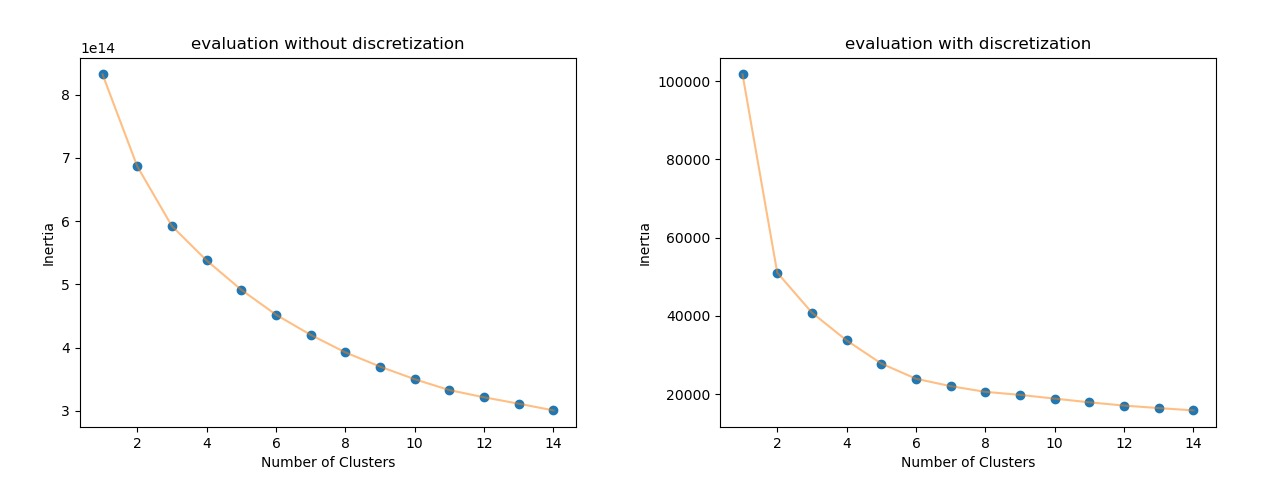
\includegraphics[width=1\columnwidth]{figures/Kmeans_K.jpg}
    \caption{K means, variazione del numero di k cluster}
    \label{fig:k_means1}
\end{figure}
\begin{figure}[H]
    \centering
    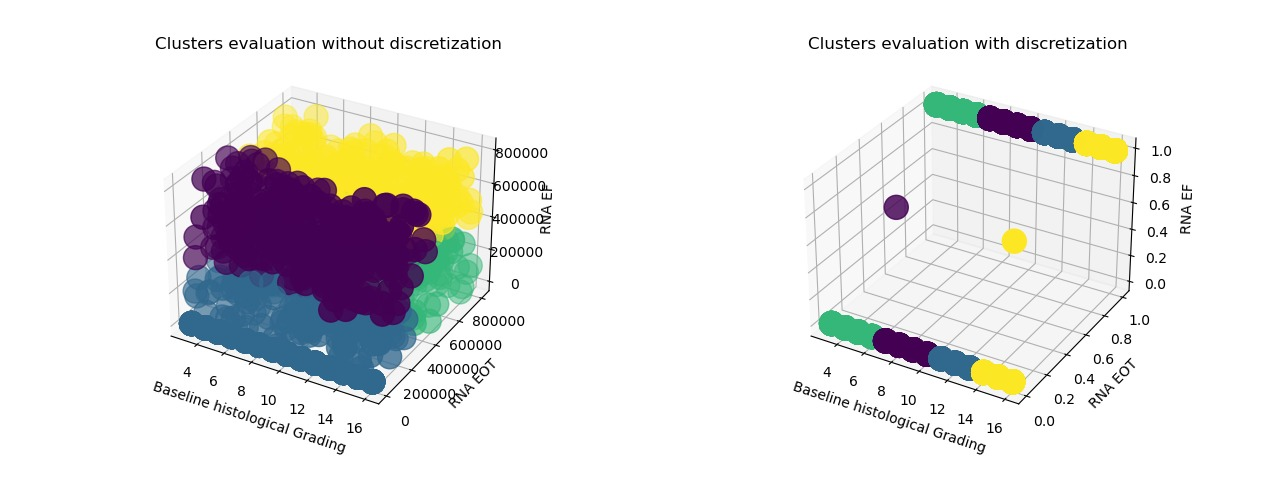
\includegraphics[width=1\columnwidth]{figures/clusters.jpg}
    \caption{Plot 3D del clustering con 3 features}
    \label{fig:k_means2}
\end{figure}

\subsection{Criterio di Splitting del dataset}

Ho voluto riservare al Training set, ovvero la porzione di dati su cui i modelli si addestreranno, un 80\% mentre per il Test set per la valutazione dei risultati un 20\%. Quindi 1.108 su 1385 samples sono riservati al training e 277 per il test.

\begin{figure}[H]
    \centering
    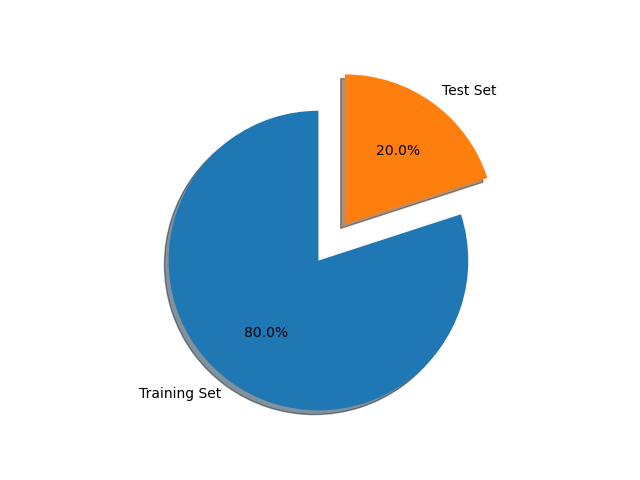
\includegraphics[width=0.75\columnwidth]{figures/pieSplitting.png}
    \caption{Splitting}
    \label{fig:splitting}
\end{figure}

    



